%%%%%%%%%%%%%%%%%%%%%%%%%%%%%%%%%%%%%%%%%%%%%%%%%%%%%%%%%%%%%%%%%%%%%%
% Problem statement
\begin{statement}[
  problempoints=110,
  timelimit=2 seconds,
  memorylimit=256 MiB,
]{Holding}

\setlength\intextsep{-0.1cm}
\begin{wrapfigure}[9]{r}{0.17\textwidth}
\centering
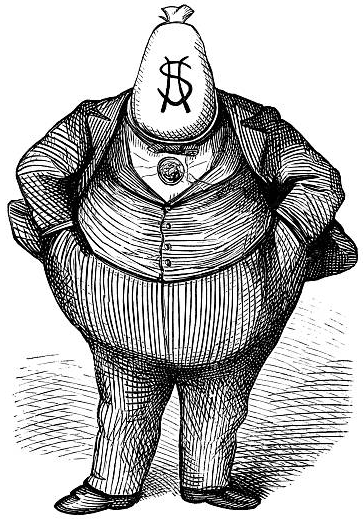
\includegraphics[width=0.17\textwidth]{img/holding.png}
\end{wrapfigure}

Difficult times lie ahead of Ivica and his Holding -- a group of $N$ Croatian
companies that are in his ownership. Each of these companies is in debt so the
state sent its attorneys to take everything away from him. We have exclusively
found out that Ivica managed to make a deal with the state to leave him certain
companies in spite of the massive debt. Which ones? We found that out as well.

The state attorneys have laid out $N$ proprietary papers of Ivica's companies
on the table.  The debt of first company is written on the first paper $A_1$,
the debt of the second company is written on $A_2$, \dots and the debt of the
last company is written on the last paper $A_N$. Ivica made a deal with the
state to leave the companies $A_L$, $A_{L+1}$, \dots , $A_R$ in his
ownership, where $L$ and $R$ represent the positions in an array of papers on
the table.  Fortunately for Ivica, the attorneys are (also) corrupt. They
will force him to take the same contiguous subarray as agreed upon (from
$L$-th to $R$-th paper), but they will let him swap any two papers on the
table for a specific cost. More precisely, swapping papers at positions $i$
and $j$ will cost him $|i-j|$ kunas (Croatian currency).  Ivica is desperate.
He has only $K$ kunas in his pocket which he now wishes to spend in such a
way that the sum of debts of companies he is left with is as small as
possible.

Help Ivica achieve his goal.

%%%%%%%%%%%%%%%%%%%%%%%%%%%%%%%%%%%%%%%%%%%%%%%%%%%%%%%%%%%%%%%%%%%%%%
% Input
\subsection*{Input}
The first line contains four space-separated integers $N$, $L$, $R$
$(1 \le L \le R \le N \le 100)$ and $K$ $(0 \le K \le 10\ 000)$ from the
task description.

The second line contains $N$ integers $A_i$ $(0 \le A_i \le 10^6)$  from
the task description.

%%%%%%%%%%%%%%%%%%%%%%%%%%%%%%%%%%%%%%%%%%%%%%%%%%%%%%%%%%%%%%%%%%%%%%
% Output
\subsection*{Output}
You should output a single integer which represents the smallest amount of
total debt Ivica will have if he spends his $K$ kunas optimally.

%%%%%%%%%%%%%%%%%%%%%%%%%%%%%%%%%%%%%%%%%%%%%%%%%%%%%%%%%%%%%%%%%%%%%%
% Scoring
 \subsection*{Scoring}
{\renewcommand{\arraystretch}{1.4}
  \setlength{\tabcolsep}{6pt}
  \begin{tabular}{ccl}
 Subtask & Score & Constraints \\ \midrule
  1 & 22 & $N \le 13$ and $R = N$ \\
  2 & 33 & $N \le 50$ and $R = N$  \\
  3 & 33 & $N \le 50$ \\
  4 & 22 & No additional constraints.
\end{tabular}}

%%%%%%%%%%%%%%%%%%%%%%%%%%%%%%%%%%%%%%%%%%%%%%%%%%%%%%%%%%%%%%%%%%%%%%
% Examples
\subsection*{Examples}
\begin{tabularx}{\textwidth}{X'X'X}
\sampleinputs{test/holding.dummy.in.1}{test/holding.dummy.out.1} &
\sampleinputs{test/holding.dummy.in.2}{test/holding.dummy.out.2} &
\sampleinputs{test/holding.dummy.in.3}{test/holding.dummy.out.3}
\end{tabularx}

%%%%%%%%%%%%%%%%%%%%%%%%%%%%%%%%%%%%%%%%%%%%%%%%%%%%%%%%%%%%%%%%%%%%%%
% We're done
\end{statement}

%%% Local Variables:
%%% mode: latex
%%% mode: flyspell
%%% ispell-local-dictionary: "croatian"
%%% TeX-master: "../hio.tex"
%%% End:
